\chapter{Arquitetura e Tecnologias}

No presente tópico, são definidas e detalhadas todas as partes que envolvem a arquitetura e tecnologias utilizadas no sistema. Nesse sentido, modelos visuais foram criados com o propósito de proporcionar um melhor entendimento e assimilação do funcionamento do sistema.

\section{Escopo do Projeto}

No escopo, busca-se compreender a extensão do projeto e todas as partes abrangidas por ele, tanto no âmbito do negócio quanto no âmbito do desenvolvimento. Adicionalmente, são destacadas as metas e objetivos do desenvolvimento nesta seção.

% Requisitos
\subsection{Requisitos}

Neste tópico, são analisados e definidos os fatores de negócio do projeto, tais como requisitos funcionais, requisitos não funcionais, regras de negócio, histórias de usuários e possíveis casos de uso. Todos esses fatores foram considerados para o desenvolvimento do projeto e devem ser seguidos de maneira objetiva e concreta. É importante ressaltar que determinados requisitos e histórias podem sofrer alterações no futuro, uma vez que mudanças no projeto podem ocorrer.

% Regras de negócio
\subsubsection{Regras de Negócio}
\label{sec:regras_negocio}

Os Quadros \ref{tab:regrasdenegocio1}, \ref{tab:regrasdenegocio2} e \ref{tab:regrasdenegocio3} estão organizados por temas, com o propósito de aprimorar a organização e a compreensão do conteúdo. Estes quadros têm como objetivo descrever de maneira abrangente todas as regras de negócio propostas, as quais devem ser integralmente incorporadas nos requisitos funcionais e não funcionais do projeto.

\begin{quadro}[h!]
\centering
\caption{Regras de Negócio de Login, Autenticação e Usuário}
\label{tab:regrasdenegocio1}
\begin{longtable}{|p{2.5cm}|p{10.0cm}|p{2.5cm}|}
\hline
ID & Descrição & Relacionados
\\\hline
RN1 & Ao acessar o site, para ter acesso aos conteúdos e funcionalidades, o usuário deve estar previamente autenticado &  \
\\\hline
RN2 & O acesso do usuário ao sistema de login é restrito àqueles que possuem um cadastro ativo &  \
\\\hline
RN3 & Durante o processo de cadastro, é imprescindível que o usuário confirme seu endereço de e-mail a fim de validar seu registro &  \
\\\hline
RN4 & Deve ser enviado um e-mail para redefinição de senhas de usuários &  \
\\\hline
RN5 & Cada usuário deve possuir um perfil individual, através do qual poderá administrar seus dados pessoais e informações relacionadas aos jogos &  \
\\\hline
RN6 & O usuário possui a prerrogativa de editar seus próprios dados pessoais &  \
\\\hline
RN7 & É facultado ao usuário o direito de excluir sua conta a qualquer momento &  \
\\\hline
\end{longtable}
\fonte{Os Autores.}
\end{quadro}

\begin{quadro}[h!]
\centering
\caption{Regras de Negócio de Gerenciamento de Jogos e Assinatura Premium}
\label{tab:regrasdenegocio2}
\begin{longtable}{|p{2.5cm}|p{10.0cm}|p{2.5cm}|}
\hline
ID & Descrição & Relacionados
\\\hline
RN8 & Ao selecionar um jogo, o usuário tem a possibilidade de adicioná-lo ao seu perfil &  \
\\\hline
RN9 & No momento de adicionar o jogo, é exigido que o usuário forneça informações básicas sobre o jogo &  \
\\\hline
RN10 & Após a inclusão, o usuário terá permissão para editar as informações dos seus jogos &  \
\\\hline
RN11 & No perfil do usuário, devem estar disponíveis todas as listagens de jogos, organizadas com base em seu status &  \
\\\hline
RN12 & Os usuários devem ter a capacidade de visualizar todos os jogos e avaliações nos perfis de outros usuários &  \
\\\hline
RN13 & O usuário terá a opção de filtrar os jogos com base em determinados parâmetros &  \
\\\hline
RN14 & O usuário deve ser capaz de avaliar um jogo, atribuindo uma nota e fornecendo uma crítica &  \
\\\hline
RN15 & O usuário deve ter a capacidade de excluir os jogos que adicionou a qualquer momento &  \
\\\hline
RN16 & Os usuários serão categorizados em usuários comuns e usuários premium &  \
\\\hline
RN17 & O sistema deve incorporar um modelo de assinatura premium, onde os usuários que pagarem uma quantia específica terão acesso a determinados benefícios e funcionalidades exclusivas &  \
\\\hline
RN18 & Usuários comuns não terão acesso a benefícios extras &  \
\\\hline
RN19 & Os usuários premium têm o direito de cancelar sua assinatura a qualquer momento &  \
\\\hline
\end{longtable}
\fonte{Os Autores.}
\end{quadro}


\begin{quadro}
\centering
\caption{Regras de Negócio da Arena de Jogos}
\label{tab:regrasdenegocio3}
\begin{longtable}{|p{2.5cm}|p{10.0cm}|p{2.5cm}|}
\hline
ID & Descrição & Relacionados
\\\hline
RN20 & O sistema deve oferecer uma aba dedicada às arenas &  \
\\\hline
RN21 & Cada arena deve possuir um administrador designado, sendo restrito aos usuários premium o direito de se tornarem administradores de arenas &  \
\\\hline
RN22 & Ao criar uma arena, o administrador é responsável por definir informações essenciais, como o jogo a ser jogado e a descrição da arena &  \
\\\hline
RN23 & O administrador tem a autorização para excluir sua arena a qualquer momento &  \
\\\hline
RN24 & Cada arena contará com um chat exclusivo, permitindo a comunicação entre todos os jogadores presentes na arena &  \
\\\hline
\end{longtable}
\fonte{Os Autores.}
\end{quadro}
\pagebreak

% Requisitos funcionais
\clearpage
\subsubsection{Requisitos Funcionais}
\label{sec:req_funcionais}

Neste capítulo, apresentam-se os requisitos indispensáveis à garantia de usabilidade e prestação de serviço abrangente aos usuários da aplicação. A síntese destes requisitos é fornecida nos Quadros \ref{tab:requisitosfuncionais1} e \ref{tab:requisitosfuncionais2}, onde se estabelece uma visão panorâmica dessas demandas. Estes quadros contextualizam os requisitos com as regras de negócio correspondentes e destacam a sua relevância no contexto do desenvolvimento, crucial para assegurar o sucesso do projeto.

\begin{quadro}[h!]
\caption{Requisitos Funcionais de Login, Usuário e Gerenciamento de Jogos}
\label{tab:requisitosfuncionais1}
\begin{longtable}{|p{2.5cm}|p{7.5cm}|p{2.5cm}|p{2.5cm}|}
\hline
ID & Descrição & Importância & Relacionados
\\\hline
RF1 & O sistema deve permitir que novos usuários realizem o cadastro & Alta & RN3 \
\\\hline
RF2 & O sistema deve permitir que os usuários realizem o login & Alta & RN2 \
\\\hline
RF3 & O sistema deve ser capaz de enviar um e-mail para confirmação de conta & Alta & RN3 \
\\\hline
RF4 & O sistema deve impedir o acesso a recursos por usuários não autenticados & Alta & RN1 \
\\\hline
RF5 & O sistema deve possibilitar que os usuários alterem suas senhas & Média & RN4 \
\\\hline
RF6 & O sistema deve possibilitar ao usuário a edição de seus dados pessoais e a exclusão de sua conta & Média & RN5, RN6, RN7 \
\\\hline
RF7 & O sistema deve possibilitar que o usuário adicione, edite e remova um jogo do seu perfil & Alta & RN5, RN8, RN9, RN10, RN15 \
\\\hline
RF8 & O sistema deve permitir que os usuários avaliem jogos, atribuindo uma nota e fornecendo uma crítica sobre sua experiência com o jogo & Alta & RN14 \
\\\hline
RF9 & O sistema deve exibir uma lista de jogos no perfil do usuário, organizada por status & Média & RN11 \
\\\hline
RF10 & O sistema deve permitir que os usuários pesquisem por outros perfis e acessem esses perfis & Média & RN12 \
\\\hline
RF11 & O sistema deve oferecer opções de filtro nas listagens de jogos & Média & RN13 \
\\\hline
\end{longtable}
\fonte{Os Autores.}
\end{quadro}

\begin{quadro}[h!]
\caption{Requisitos Funcionais de Assinatura Premium e Arena}
\label{tab:requisitosfuncionais2}
\begin{longtable}{|p{2.5cm}|p{7.5cm}|p{2.5cm}|p{2.5cm}|}
\hline
ID & Descrição & Importância & Relacionados
\\\hline
RF12 & O sistema deve oferecer uma aba que apresente os tipos de planos de usuários disponíveis & Alta & RN17 \
\\\hline
RF13 & O sistema deve possibilitar que um usuário assine o plano premium ou cancele sua assinatura a qualquer momento & Alta & RN16, RN18, RN19 \
\\\hline
RF14 & O sistema deve incluir uma aba que apresente todas as arenas de jogos disponíveis & Alta & RN20 \
\\\hline
RF15 & O sistema deve permitir que usuários premium criem e removam suas próprias arenas de jogos & Alta & RN21, RN22, RN23 \
\\\hline
RF16 & O sistema deve disponibilizar um chat de comunicação para os usuários da arena. & Alta & RN24 \
\\\hline
\end{longtable}
\fonte{Os Autores.}
\end{quadro}
\pagebreak

% Requisitos não funcionais
\pagebreak
\subsubsection{Requisitos Não Funcionais}
\label{sec:req_nao_funcinais}

O Quadro \ref{tab:requisitosnaofuncionais} busca elucidar os requisitos não funcionais do sistema, estabelecendo uma correlação entre cada um desses requisitos e a sua relevância intrínseca no âmbito do desenvolvimento.

\begin{quadro}[h!]
\centering
\caption{Requisitos Não Funcionais}
\label{tab:requisitosnaofuncionais}
\begin{longtable}{|p{2.5cm}|p{10.0cm}|p{2.5cm}|}
\hline
ID & Descrição & Importância
\\\hline
RNF1 & A interface do sistema deve ser objetiva e de fácil usabilidade & Alta
\\\hline
RNF2 & O sistema deve possuir interfaces responsivas & Alta
\\\hline
RNF3 & O sistema deve estar em conformidade com a \ac{lgpd} & Alta
\\\hline
RNF4 & O sistema deve estar disponível para uso 24 horas por dia, todos os dias da semana & Alta
\\\hline
RNF5 & O sistema deve possuir uma comunicação eficiente e rápida entre suas partes & Alta
\\\hline
\end{longtable}
\fonte{Os Autores.}
\end{quadro}
\pagebreak

% Arquitetura
\section{Arquitetura}

Nesta seção, proporciona-se uma visão abrangente da arquitetura da aplicação, englobando os padrões e princípios de design adotados na concepção da solução. Além disso, são detalhadas as tecnologias, \textit{\gls{Frameworks}} e bibliotecas utilizados no desenvolvimento da aplicação, acompanhados das considerações referentes à segurança e escalabilidade incorporadas na arquitetura da solução.

\subsection{Desenho da aplicação}

Para o projeto em questão, adotou-se uma abordagem convencional de arquitetura web cliente-servidor, em que a interface \textit{\gls{Front-end}} se interconecta com a \ac{api} \textit{\gls{Back-end}} por meio dos protocolos HTTP disponíveis. É crucial ressaltar que uma \ac{api} externa fornecida pela \textit{\gls{Rawg}} foi empregada, ampliando significativamente a disponibilidade de informações acerca de jogos, como datas de lançamento, avaliações, plataformas e outros dados relevantes. Além disso, foi utilizada a \ac{api} do \gls{MercadoPago} para auxiliar no processamento de transações monetárias para as assinaturas premium. A Figura \ref{DesenhoArquitetura} oferece uma representação completa do diagrama arquitetural implementado no sistema.

\begin{figure}[H]
    \centering
	\caption{Desenho da Arquitetura}
    \label{DesenhoArquitetura}
    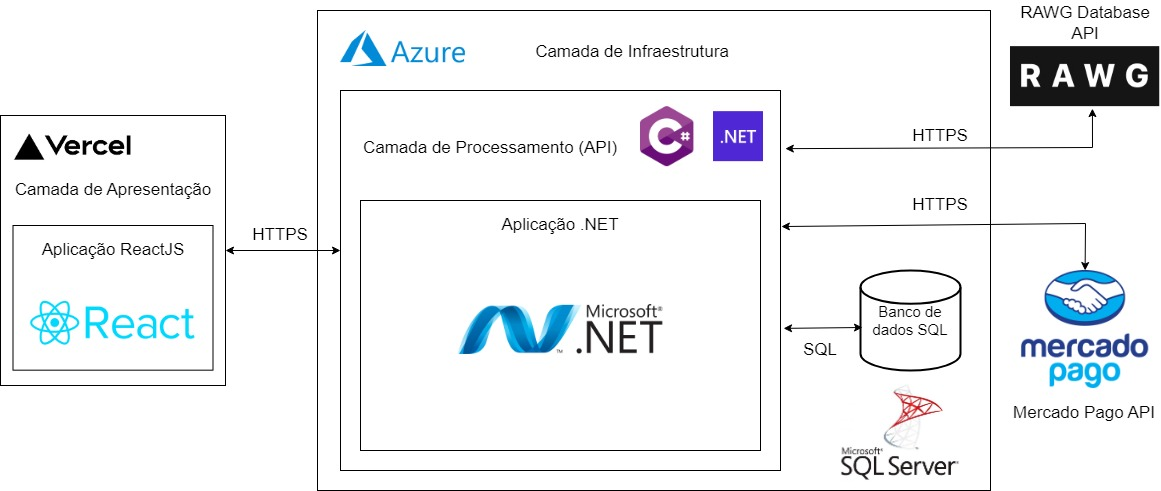
\includegraphics[scale = 0.37]{imagens/arquitetura/desenho_arquitetura.jpg}	
    \fonte{Os Autores}
\end{figure}

% Tecnologias e Ferramentas
\subsection{Tecnologias}

Nesta seção, apresentar-se-á uma visão geral de todas as tecnologias escolhidas para a implementação da aplicação, incluindo as linguagens de programação, \textit{\gls{Framework}} e bibliotecas utilizadas.

\subsubsection{Back-end}

No âmbito do \textit{\gls{Back-end}}, a escolha recaiu sobre a linguagem de programação \textit{\gls{Csharp}}, em concomitância com a plataforma de desenvolvimento e o \textit{Framework} \textit{\gls{.NET}}. Por conseguinte, foi concebida uma \ac{api} voltada ao gerenciamento da aplicação e à manipulação dos dados. No tocante à criação das tabelas do banco de dados e à gestão dos dados existentes, recorreu-se ao pacote \textit{\gls{Entity}}, que desempenha a função de \ac{orm} no âmbito deste projeto.

\subsubsection{Front-end}

No contexto do desenvolvimento do \textit{\gls{Front-end}} da aplicação, a linguagem de programação \textit{\gls{Javascript}} foi selecionada, em conjunto com a biblioteca \textit{\gls{React}}, para a construção dos componentes essenciais da plataforma. Adicionalmente, o \ac{css} foi empregado para conferir estilo às páginas, visando aprimorar a atratividade visual das interfaces aos olhos dos usuários. Por último, foram incorporadas bibliotecas destinadas a animação e ao controle de formulários, com o propósito de proporcionar suporte e otimizar a condução do processo de desenvolvimento da aplicação.

\subsubsection{Banco de dados}

Para a gestão e acesso aos dados, a opção recaiu sobre o \textit{\gls{Sqlserver}}, utilizando uma instância fornecida pelo serviço Azure. No processo de estruturação das tabelas e aplicação das etapas de normalização, a escolha foi direcionada à utilização do pacote \textit{\gls{Entity}}, desenvolvido pela \textit{\gls{Microsoft}}.

\subsubsection{Infraestrutura}

Quanto ao processo de \textit{\gls{Deploy}} da aplicação, é importante ressaltar que o \textit{\gls{Front-end}} foi devidamente hospedado na plataforma \textit{\gls{Vercel}}, enquanto o \textit{\gls{Back-end}} na plataforma da \textit{\gls{Azure}}.

\subsubsection{Escalabilidade}

As ferramentas disponibilizadas pela plataforma \textit{\gls{Azure}} foram empregadas no decorrer deste projeto, notadamente o sistema de dimensionamento automático. Tal emprego teve por objetivo primordial a adequação dinâmica da aplicação, alinhando-a de maneira precisa às demandas e necessidades apresentadas.

\subsubsection{APIs Externas}
Foram utilizadas duas \ac{api} externas para fornecer recursos e ferramentas à aplicação, sendo uma pertencente à \textit{\gls{Rawg}} e a outra, ao \gls{MercadoPago}.

A \ac{api} da \textit{\gls{Rawg}} foi utilizada por fornecer um
vasto conjunto de informações pertinentes ao universo dos jogos digitais, abrangendo
aspectos como o ano de lançamento, o estúdio desenvolvedor, os criadores e outros detalhes
relevantes.

Já a \ac{api} do \gls{MercadoPago} foi empregada para fornecer apoio ao fluxo de pagamento do plano premium fornecido pela aplicação, já que ela traz consigo todos os recursos necessários para realizar essas transações de forma segura.

% Critérios de Segurança/Privacidade/Legislação
\section{Critérios de Segurança/Privacidade/Legislação}
Esta seção tem como objetivo descrever, em termos gerais, os elementos de segurança implementados no projeto, bem como os critérios de privacidade seguidos e uma visão geral sobre seu enquadramento nos requisitos da \ac{lgpd}.

\subsection{Segurança Implantada para API Externa}

A obtenção de acesso à API da \textit{\gls{Rawg}} demanda a alocação de um domínio de site associado e, por este motivo, o domínio da \textit{GameLocker} foi estabelecido para esse propósito específico. Adicionalmente, como parte desse processo, foi criada uma chave de autenticação, a qual é necessária para ser inclusa em todas as requisições direcionadas à \ac{api}.

Nesse contexto, surge a necessidade de garantir a segurança da chave de autenticação. Tradicionalmente, as requisições à \ac{api} externa são efetuadas a partir do \textit{\gls{Front-end}} do projeto. No entanto, na presente situação, devido à sensibilidade da chave de autenticação, medidas adicionais se tornaram essenciais. Permitir que qualquer usuário do site a obtenha ao realizar requisições à \textit{GameLocker} seria um risco considerável.

Portanto, com a segurança em destaque, a decisão unânime foi a de implementar as requisições à \ac{api} da \textit{\gls{Rawg}} por meio do \textit{\gls{Back-end}}. Esse enfoque se revelou crucial para salvaguardar a chave de autenticação. Ao adotar essa abordagem, a chave não fica exposta às requisições realizadas pelos usuários no site, mitigando a possibilidade de utilização maliciosa. Em síntese, essa estratégia se alinha com as melhores práticas de segurança, garantindo a integridade e a confidencialidade da chave de autenticação, assim como a proteção do projeto em relação a potenciais atividades maliciosas.

\subsection{Segurança no Back-end}

Toda aplicação que almeja conquistar uma posição no mercado atual deve imperativamente oferecer uma camada de segurança robusta, com ênfase na autorização e autenticação de usuários. Nesse contexto, é fundamental reiterar que a autenticação consiste na validação da identidade de um usuário, assegurando a correspondência entre a alegação de identidade e a real identificação. Paralelamente, a autorização se refere aos recursos específicos que um usuário autenticado está habilitado a acessar.

Na \ac{api} concebida com a utilização da tecnologia \textit{\gls{.NET}}, optou-se por integrar o pacote \textit{\gls{Identity}}, desenvolvido e mantido pela \textit{\gls{Microsoft}}. O \textit{\gls{Identity}} oferece uma ampla gama de funcionalidades que simplificam a incorporação e o uso de sistemas de autenticação e autorização no contexto da aplicação. O primeiro aspecto de segurança abordado no âmbito do \textit{\gls{Back-end}} está relacionado ao procedimento de cadastro de usuários, o qual contempla diversas dimensões cruciais em termos de segurança.

Um exemplo notável é a exigência de que a senha atenda a critérios predefinidos, garantindo a solidez do registro do usuário na plataforma. Uma vez concluído o cadastro, o usuário é conduzido ao processo de autenticação no sistema, utilizando suas credenciais de e-mail e senha. É relevante destacar que os endereços de e-mail são exclusivos no ambiente da aplicação, sendo que a efetivação do login somente é possível mediante o fornecimento das credenciais precisas.

Com o êxito na autenticação, o sistema gera um componente de importância ímpar para o \textit{\gls{Front-end}} do projeto, denominado \textit{token} de autenticação do usuário. Visando assegurar uma proteção amplificada da aplicação, o acesso a qualquer recurso na \ac{api} do projeto requer a submissão do \textit{token} correspondente ao usuário. Tal \textit{token} é então validado no âmbito do \textit{\gls{Back-end}} do sistema, garantindo a integridade do processo de autorização e a salvaguarda dos recursos acessados.

\subsection{Segurança no Front-End}

No âmbito do desenvolvimento da aplicação, a segurança referente ao \textit{\gls{Front-end}} foi abordada com seriedade e profissionalismo, sendo implementadas uma série de medidas para salvaguardar informações pessoais e preservar a integridade das contas dos usuários. A seguir, são apresentadas algumas das principais ações de segurança adotadas:

\begin{itemize}
    \item Autenticação Convencional: Foi adotado um sistema de cadastro e login convencional para autenticar os usuários. Tal abordagem exige que cada usuário crie uma conta exclusiva com um nome de usuário e senha. As senhas são armazenadas de maneira criptografada no banco de dados, o que previne acessos não autorizados, garantindo a proteção da informação;
\end{itemize}

\begin{itemize}
    \item Certificado \ac{ssl}: A aplicação incorpora um certificado \ac{ssl} para estabelecer uma conexão segura entre o navegador do usuário e o servidor. Essa camada adicional de segurança cifra as informações transmitidas, incluindo dados pessoais e credenciais de login, para impedir qualquer tentativa de interceptação por terceiros mal-intencionados. A utilização do \ac{ssl} promove a confidencialidade e a integridade dos dados durante a interação entre o usuário e o servidor;
\end{itemize}

\begin{itemize}
    \item Protocolo \ac{https}: O protocolo \ac{https} foi adotado para todas as transações efetuadas no site. O \ac{https} é uma variante segura do protocolo \ac{http}, e sua presença indica que a comunicação entre o navegador do usuário e o servidor está protegida por criptografia. Esse enfoque resguarda as informações em trânsito, impedindo qualquer interceptação ou manipulação indesejada.
\end{itemize}

Adicionalmente a essas iniciativas, foram implementadas outras práticas de segurança recomendadas, incluindo atualizações regulares do software tanto do site quanto do servidor. Além disso, um sistema de monitoramento para detectar atividades suspeitas foi estabelecido, aprimorando a proteção e a vigilância contínua do ambiente digital.

\subsection{Segurança nos Repositórios}

O projeto é constituído por dois repositórios, nos quais os códigos do projeto são alocados e conservados. Enquanto um destes repositórios acolhe o código do \textit{\gls{Back-end}}, o outro desempenha a função de custodiar o código do \textit{\gls{Front-end}}. Com a finalidade de salvaguardar a integridade desses repositórios, eles são configurados como privados, uma medida que atua como uma barreira eficaz contra acessos, visualizações ou modificações por parte de indivíduos externos. Destarte, somente os membros integrantes do projeto ostentam a prerrogativa de autorização para adentrar e utilizar os recursos embutidos nesses repositórios.

\subsection{Segurança no Azure}

O processo de \textit{\gls{Deploy}} do projeto é executado através da plataforma de computação em nuvem da \textit{\gls{Azure}}. A própria plataforma \textit{\gls{Azure}} disponibiliza uma série de recursos dedicados à segurança para seus usuários, e esses recursos são integralmente empregados no âmbito deste projeto.

O primeiro recurso destaca-se por assegurar a proteção do acesso aos serviços hospedados na nuvem. Essa salvaguarda é estabelecida ao restringir o acesso somente a pontos críticos e essenciais, consolidando assim a salvaguarda dos serviços associados ao projeto.

Adicionalmente, uma segunda medida de segurança é aplicada através da limitação do \textit{\gls{Deploy}} do projeto na plataforma \textit{\gls{Azure}} exclusivamente para as máquinas que pertencem aos membros participantes do projeto. Essa estratégia contribui para acrescentar uma camada adicional de proteção ao processo de \textit{\gls{Deploy}}, mitigando potenciais riscos ao controlar estritamente o escopo das máquinas autorizadas a realizar o \textit{\gls{Deploy}} na plataforma.

\subsection{Lei Geral de Proteção de Dados}
A \ac{lgpd}, de acordo com o Congresso Nacional, "(...) dispõe sobre o tratamento de dados pessoais, inclusive nos meios digitais, por pessoa natural ou por pessoa jurídica de direito público ou privado, com o objetivo de proteger os direitos fundamentais de liberdade e de privacidade e o livre desenvolvimento da personalidade da pessoa natural." \cite{lgpd}.

Portanto, durante o desenvolvimento do projeto, foram tomadas decisões e
medidas de segurança para que ele se encaixasse e estivesse em conformidade com essa legislação, tendo foco em uma experiência segura para os usuários.

Os dados pessoais coletados para o cadastro, que são: nome completo, \textit{email}, telefone e data de nascimento, não se enquadram como dados pessoais sensíveis segundo o Art. 5°, II da \ac{lgpd} e, por este motivo, grande parte das restrições legislativas impostas não afetam diretamente o projeto.

Além disso, a aplicação permite o acesso aos dados pessoais fornecidos, bem como sua alteração, enquadrando-se no princípio de boa-fé do livre acesso aos dados, definido no Art. 6°,IV. A aplicação requisitará consentimento dos usuários para armazenar os dados fornecidos e manipulá-los como necessário para o funcionamento do sistema, o que confere a ela conformidade com o Art. 7°,I e Art. 6°,I.

Nos apêndices deste documento, no capítulo \ref{termos-e-condicoes}, estão detalhados os termos e condições com os quais o usuário precisará concordar para utilizar a aplicação.

% Documentação da API (Swagger)
\section{Documentação}

Uma documentação bem elaborada proporciona inúmeros benefícios para o desenvolvimento de projetos na área da tecnologia. No caso da \ac{api} desenvolvida em \textit{\gls{.NET}}, a documentação das suas rotas de acesso foi realizada por meio do \textit{\gls{Swagger}}, com o objetivo de facilitar o entendimento de cada rota e sua função no sistema.

A imagem inaugural aborda de maneira específica as rotas correspondentes aos mecanismos de acesso e ao gerenciamento da conta do usuário. Estes \textit{\gls{Endpoints}} podem ser observados com clareza na Figura \ref{RotasAccount}, sendo que cada um é acompanhado por uma exposição elucidativa acerca do propósito subjacente de sua funcionalidade.

\begin{figure}[H]
    \centering
	\caption{Rotas do Usuário}
    \label{RotasAccount}
    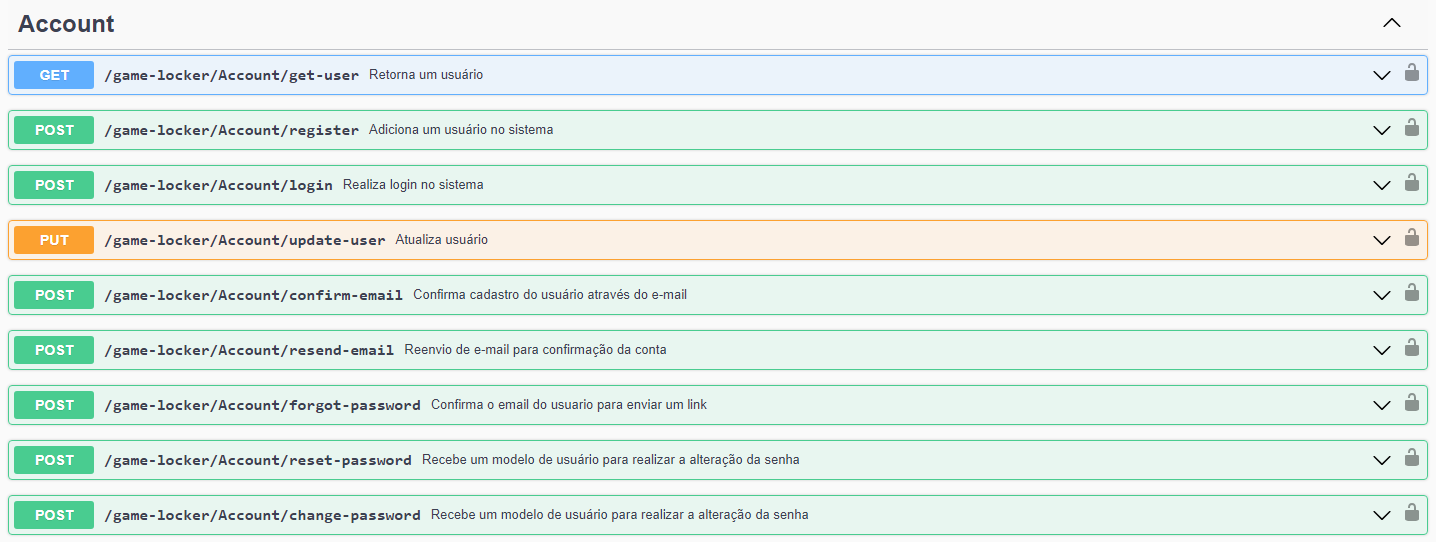
\includegraphics[scale = 0.38]{imagens/arquitetura/rotas_account.png}	
    \fonte{Os Autores}
\end{figure}

A segunda representação gráfica ilustra de maneira distintiva a rota destinada ao acesso a uma \ac{api} externa fornecida pela \textit{\gls{Rawg}}. É imperativo enfatizar que esta invocação à \ac{api} externa ocorre de modo exclusivo no \textit{\gls{Back-end}}, uma precaução tomada em virtude das considerações de segurança inerentes à aplicação. A Figura \ref{RotasApi} proporciona uma visualização precisa dessa rota singular, oferecendo uma compreensão nítida do seu papel e relevância intrínseca no contexto da arquitetura da aplicação.

\begin{figure}[H]
    \centering
	\caption{Rota da API externa}
    \label{RotasApi}
    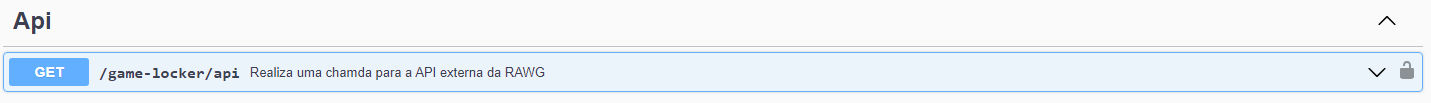
\includegraphics[scale = 0.38]{imagens/arquitetura/rotas_api.png}	
    \fonte{Os Autores}
\end{figure}

A terceira representação gráfica fornece uma visão abrangente de todas as rotas relacionadas às \gls{Review} no âmbito da aplicação. Esta seção assume um papel central na aplicação, demandando, assim, uma ênfase adicional em termos de considerações. A Figura \ref{RotasReview} elucida essas rotas de maneira detalhada, delineando as respectivas funcionalidades que desempenham no contexto do projeto.

\begin{figure}[H]
    \centering
	\caption{Rotas de Review}
    \label{RotasReview}
    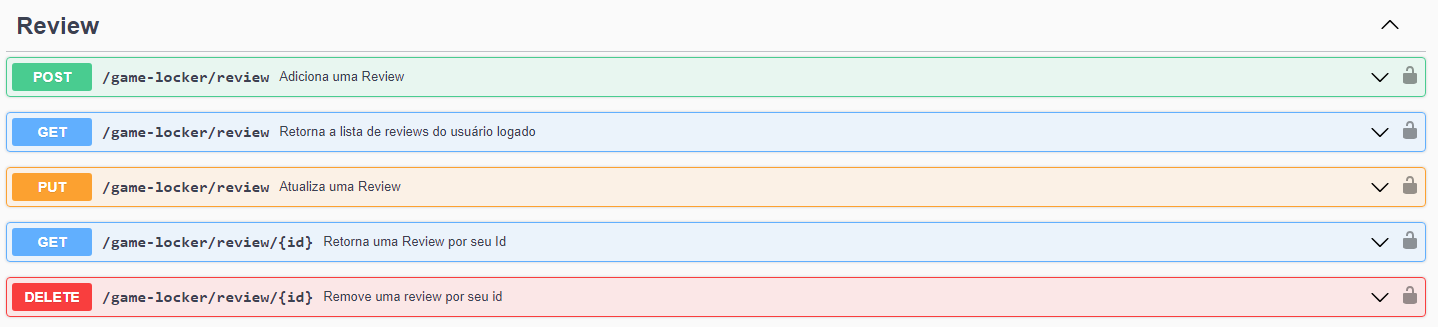
\includegraphics[scale = 0.38]{imagens/arquitetura/rotas_review.png}	
    \fonte{Os Autores}
\end{figure}

A figura \ref{RotasArena} descreve as rotas relacionadas à Arena de Jogos da Aplicação, fornecendo um panorama geral sobre as responsabilidades dessas rotas.

\begin{figure}[H]
    \centering
	\caption{Rotas de Arena}
    \label{RotasArena}
    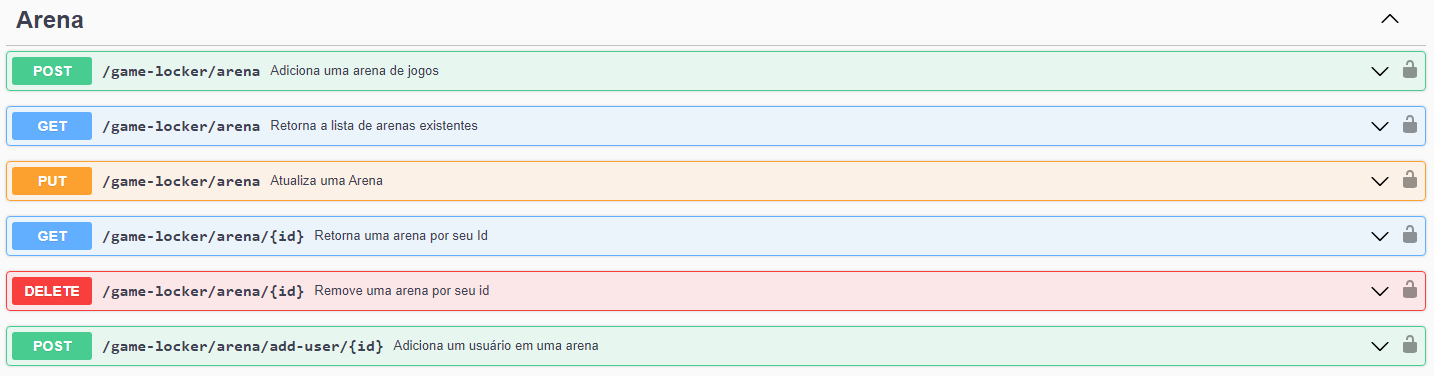
\includegraphics[scale = 0.38]{imagens/arquitetura/rotas_arena.png}	
    \fonte{Os Autores}
\end{figure}

Na figura \ref{RotasPayment} descreve as rotas que interagem diretamente com a \ac{api} do \gls{MercadoPago}, permitindo que as transações sejam realizadas de maneira segura no momento de adesão ao plano premium fornecido na plataforma.

\begin{figure}[H]
    \centering
	\caption{Rotas de Pagamento e Assinaturas}
    \label{RotasPayment}
    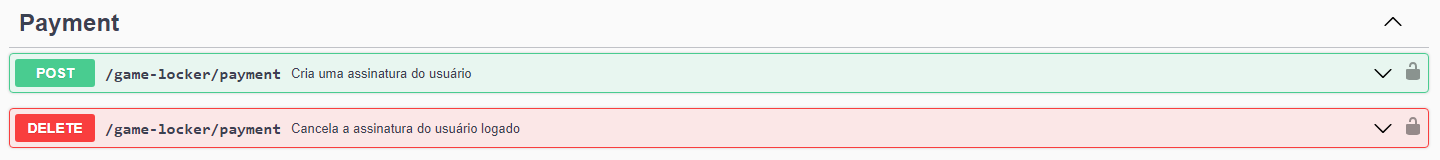
\includegraphics[scale = 0.38]{imagens/arquitetura/rotas_payment.png}	
    \fonte{Os Autores}
\end{figure}

Na Figura \ref{AutenticacaoSwagger}, encontra-se a representação da seção do \gls{Swagger} que assume a responsabilidade pela implementação da autenticação na presente \ac{api}. Importante ressaltar que todas as rotas pertencentes ao \textit{\gls{Back-end}} do projeto, com exceção das rotas de login e cadastro de contas, impõem a necessidade de autenticação para possibilitar o acesso.

\begin{figure}[H]
    \centering
	\caption{Autenticação do Swagger}
    \label{AutenticacaoSwagger}
    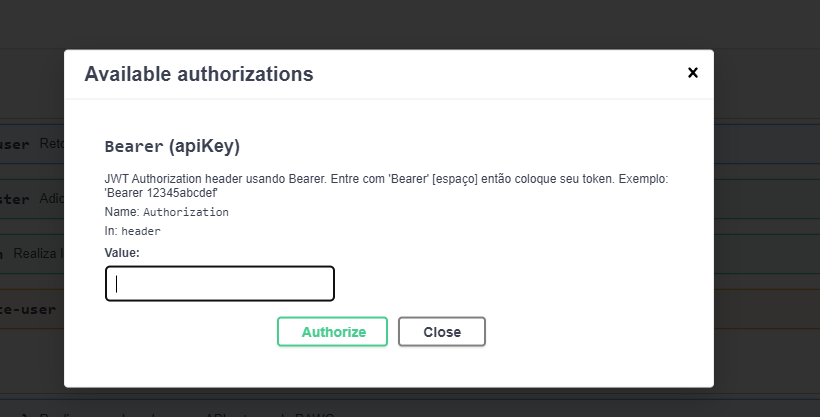
\includegraphics[scale = 0.6]{imagens/arquitetura/rotas_token.png}	
    \fonte{Os Autores}
\end{figure}

Por derradeiro, na Figura \ref{ObjetosEndpoints}, são exibidos em detalhe todos os objetos inerentes às rotas do sistema. Estes objetos carregam a responsabilidade primordial de armazenar e veicular os dados através das interações na aplicação.

\begin{figure}[H]
    \centering
	\caption{Objetos dos Endpoints}
    \label{ObjetosEndpoints}
    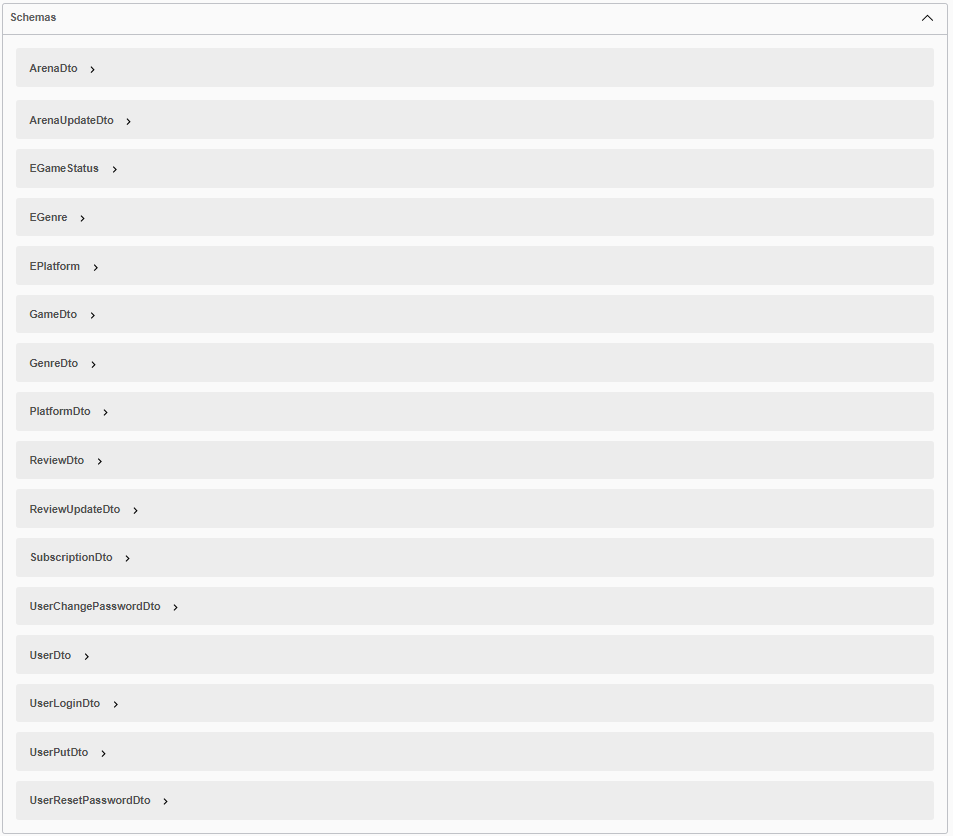
\includegraphics[scale = 0.6]{imagens/arquitetura/rotas_schemas.png}	
    \fonte{Os Autores}
\end{figure}

Para mais informações sobre a \ac{api} do projeto, consultar o link presente no capítulo \ref{LinksProjeto}, que contém este e outros links relevantes.

% Fases de Entrega
\clearpage
\section{Fases de Entrega}

Nesta seção, são estabelecidas as datas cruciais e as fases significativas do desenvolvimento do projeto, nas quais ocorrerão as entregas progressivas e escalonadas.

\subsection{Desenho da Aplicação}

No Desenho da Aplicação, foram disponibilizadas as informações essenciais para proporcionar uma compreensão abrangente tanto do projeto em si quanto da aplicação em sua totalidade. Essa entrega englobou elementos como a arquitetura, os objetivos estabelecidos e os métodos empregados no processo de desenvolvimento. O momento dessa entrega se deu no mês de abril de 2023.

\subsection{Prova de Conceito}

Na \ac{poc}, foram executadas as ações essenciais para evidenciar o funcionamento do sistema. Isso abrangeu a interligação da \ac{api} elaborada em linguagem \textit{\gls{Csharp}} e a construção da interface \textit{\gls{Front-end}} empregando a tecnologia \textit{\gls{React}}. Paralelamente, ocorreu a integração harmoniosa do sistema com a \ac{api} externa da \textit{\gls{Rawg}} e a subsequente realização do processo de implantação na plataforma \textit{\gls{Azure}}. A conclusão desta etapa ocorreu no mês de maio de 2023.

\subsection{Produto Mínimo Viável}

No \ac{mvp}, foram disponibilizadas as funcionalidades primordiais do projeto. Isso compreendeu a implementação da criação de contas e usuários, o sistema de login, bem como a validação de credenciais e identidades dos usuários. Foi igualmente elaborada uma \textit{\gls{LandingPage}} voltada para a visualização de usuários não autenticados. Além disso, um portal foi estabelecido para abarcar todos os jogos disponíveis, com funcionalidades para avaliação e observação. Destaca-se ainda a incorporação de filtros à lista de jogos, a criação de perfis de usuários e a capacidade de gerenciar jogos de forma individualizada para cada usuário. 

Este marco foi atingido no mês de junho de 2023, consolidando a entrega das bases funcionais do sistema.

\subsection{Produto}

No Produto, a entrega englobará a versão completa do projeto, abarcando integralmente todas as funcionalidades planejadas. Dentro desse rol de funcionalidades, merece destaque o desenvolvimento do sistema de arenas de jogos, a criação de chats dedicados, e a implementação da capacidade de visualizar perfis de outros usuários.

Adicionalmente, o projeto compreenderá a configuração do ciclo completo para a realização de assinaturas na aplicação, abarcando tanto a alternativa de assinatura \textit{premium} quanto a disponibilização de anúncios para os usuários comuns. A expectativa é que essa versão final seja entregue até o mês de dezembro de 2023, consolidando assim a realização plena das metas e objetivos traçados para o desenvolvimento do sistema.

% Historia de Usuario
\section{Histórias de usuário}

\begin{enumerate}
  \item \textbf{Cadastro}
  
  \textbf{Caso:} Eu, como jogador de jogos digitais, quero realizar o cadastro no site \textit{GameLocker} para fazer o gerenciamento de meus jogos e conhecer a comunidade de \textit{players}.
  
  \textbf{Critérios de Aceitação:}
  \begin{itemize}
      \item O usuário deve conseguir fazer o cadastro;
      \item O usuário deve possuir no mínimo 16 anos;
      \item E-mail do usuário deve ser único no sistema;
      \item Username do usuário deve ser único no sistema;
      \item A senha deve seguir os padrões necessários do site.
  \end{itemize}
  
  \item \textbf{Login}

  \textbf{Caso:} Eu, como jogador de jogos digitais, quero realizar o login no site GameLocker para fazer o gerenciamento de meus jogos e conhecer a comunidade de \textit{players}.
  
  \textbf{Critérios de Aceitação:}
  \begin{itemize}
      \item O usuário deve conseguir fazer o login;
      \item O usuário deve fornecer e-mail e senha corretos;
      \item O usuário não deve conseguir acessar os recursos sem estar logado;
      \item O usuário não deve conseguir fazer login com credenciais erradas.
  \end{itemize}
  
   
  \item \textbf{Adicionar Jogo/Review}

  \textbf{Caso:} Eu, como jogador de jogos digitais, quero poder adicionar a review de um jogo que estou jogando, além de oferecer uma nota e comentários para esse jogo.

  \textbf{Critérios de Aceitação:}
  \begin{itemize}
      \item O usuário deve conseguir adicionar uma review;
      \item O usuário deve conseguir colocar uma nota e um comentário para o jogo escolhido;
      \item O usuário deve selecionar um status para o jogo, o padrão deve ser jogando;
      \item O jogo adicionado pelo usuário deve ir para seu perfil.
  \end{itemize}

  \item \textbf{Visualizar reviews}

  \textbf{Caso:} Eu, como usuário que fiz reviews, quero visualizar todas minhas reviews feitas em meu perfil, para poder gerenciar elas de forma objetiva.

  \textbf{Critérios de Aceitação:}
  \begin{itemize}
      \item O usuário deve conseguir visualizar todas suas reviews;
      \item O usuário deve conseguir filtras as reviews por abas relacionadas a seus status.
  \end{itemize}

  \item \textbf{Editar Review}

  \textbf{Caso:} Eu, como usuário que adicionei uma review, quero ter a chance de editar os dados dela.

  \textbf{Critérios de Aceitação:}
  \begin{itemize}
      \item O usuário deve conseguir clicar na review escolhida e abrir um modal para editar a review;
      \item O usuário deve conseguir editar os campos liberados da review;
      \item As edições não devem ser persistidas caso o usuário não clique em salvar;
      \item Ao clicar em salvar, as edições devem ser persistidas, uma mensagem de sucesso deve aparecer e o usuário deve ser redirecionado para a listagem.
  \end{itemize}

  \item \textbf{Remover Review}

  \textbf{Caso:} Eu, como usuário que adicionei uma review errada, quero poder remover ela de forma fácil e rápida.

  \textbf{Critérios de Aceitação:}
  \begin{itemize}
      \item Ao clicar em remover, a review deve ser removida do banco de dados;
      \item Ao fazer a remoção, usuário deve ser redirecionado para a listagem atualizada.
  \end{itemize}

  \item \textbf{Filtrar Jogos Adicionados}

  \textbf{Caso:} Eu, como usuário possuo vários jogos adicionados, quero filtrar eles por nome do jogo.

  \textbf{Critérios de Aceitação:}
  \begin{itemize}
      \item Deve ter na tela uma barra de pesquisa para digitação do usuário;
      \item Filtragem deve ocorrer enquanto o usuário escreve, de forma a aparecer os resultados atualizados;
      \item Deve ter um ícone de apagar para caso o usuário queira remover o texto digitado;
      \item Ao remover o texto digitado, a listagem deve voltar ao normal;
      \item Caso não possua nenhuma correspondência para o texto digitado, deve aparecer uma mensagem informativa.
  \end{itemize}

  \item \textbf{Criar arena de jogos}

   \textbf{Caso:} Eu, como usuário premium, quero criar uma arena de um jogo para fazer um torneio entre jogadores.

   \textbf{Critérios de Aceitação:}
  \begin{itemize}
      \item Somente usuários premium podem criar arena;
      \item O administrador precisar definir algumas configurações obrigatórias no momento de criação de arena;
  \end{itemize}

  \item \textbf{Entrar na arena de jogos}

   \textbf{Caso:} Eu, como usuário que estou procurando amigos para jogar, quero entrar numa arena de algum jogo.

   \textbf{Critérios de Aceitação:}
  \begin{itemize}
      \item Deve ter a listagem de arenas disponíveis;
  \end{itemize}
  
\end{enumerate}

% Manutenibilidade
\clearpage
\section{Manutenibilidade}

Com o objetivo de garantir a longevidade da aplicação e facilitar a implementação de novas funcionalidades, torna-se crucial que a equipe de desenvolvimento siga padrões, princípios e boas práticas estabelecidos. Adicionalmente, é importante mencionar que a implementação de boas práticas não se limita apenas à codificação, mas se estende também à documentação, comunicação e colaboração entre os membros da equipe.

\subsection{Ferramentas para Testes automatizados e Análise Estática}

Para a realização dos testes automatizados no \textit{\gls{Back-end}}, será utilizado o \textit{\gls{Xunit}}, uma ferramenta de código aberto empregada para a execução de testes automatizados. Essa ferramenta oferece recursos avançados, como a paralelização de testes e a capacidade de executá-los em diversas plataformas. Além disso, o \textit{\gls{Xunit}} possui uma documentação abrangente e integração com a \ac{IDE} do \textit{\gls{VisualStudio}}, que será utilizada no desenvolvimento.

\subsection{Code Convention}

Para o desenvolvimento do \textit{\gls{Back-end}}, adotou-se a convenção de codificação da linguagem \textit{\gls{Csharp}}, conhecida como \textit{Csharp Coding Conventions}. Essa convenção foi criada e é mantida pela \textit{\gls{Microsoft}}, empresa responsável pela criação da linguagem de programação \textit{\gls{Csharp}}. É possível encontrar a documentação completa dessa convenção online. Entre as principais definições dessa convenção, destacam-se:

\begin{itemize}
\item Nomes de variáveis devem ser descritivos, utilizando-se sempre \texttt{\gls{CamelCase}} (inicia com letra minúscula);
\item Nomes de classes e tipos devem ser descritivos, iniciando com letra maiúscula e utilizando \texttt{\gls{PascalCase}};
\item Métodos devem ser nomeados utilizando verbos, seguidos de um substantivo ou frase descritiva;
\item Utilize indentação de 4 espaços, sem tabulação;
\item Chaves devem ser abertas na mesma linha que o código que as precede e fechadas em uma nova linha;
\item Cada instrução deve ser escrita em uma linha separada;
\item A largura da linha não deve ultrapassar 120 caracteres;
\item Utilize comentários em linha para explicar partes do código que possam ser difíceis de entender;
\item Use espaços em branco para separar operadores e elementos do código;
\item Utilize a palavra-chave \textit{\texttt{this}} para referenciar membros da classe atual.
\end{itemize}

Para o desenvolvimento do \textit{\gls{Front-end}}, foi utilizado o \textit{Google TypeScript Style Guide}, que é um guia de estilo de codificação para o \textit{\gls{Typescript}}, uma linguagem de programação desenvolvida pela \textit{\gls{Microsoft}}. Esse guia é mantido pelo \textit{Google} e fornece diretrizes para padronizar a escrita de código em projetos que utilizam \textit{\gls{Typescript}}.

Algumas das principais características desse guia são:

\begin{itemize}
\item Uso de \texttt{\gls{CamelCase}} para nomes de variáveis e \texttt{\gls{PascalCase}} para nomes de tipos e classes;
\item Uso de \textit{\texttt{const}} em vez de \textit{\texttt{let}} sempre que possível;
\item Uso de tipos explícitos em vez de inferência de tipos sempre que possível;
\item Evitar o uso de tipos \textit{\texttt{any}} sempre que possível;
\item Uso de \texttt{===} em vez de \texttt{==} para comparações;
\item Evitar o uso de \textit{\texttt{namespace}} e, em vez disso, utilizar módulos;
\item Uso de \texttt{interface} para definição de tipos e estruturas de objetos;
\item Utilização de apóstrofo para strings;
\item Uso de \textit{arrow functions} em vez de function expressions sempre que possível;
\item Uso de \textit{\texttt{async/await}} em vez de \textit{callbacks} para operações assíncronas.
\end{itemize}

\subsection{Integração Continua}

O \ac{ci}/\ac{cd} do GitHub é uma ferramenta amplamente utilizada em projetos de software em todo o mundo, sendo uma opção confiável e robusta para a implementação de processos de \ac{ci}/\ac{cd}. Com sua flexibilidade e facilidade de configuração, é possível acelerar a entrega de software com qualidade e eficiência.

Dentre os processos que podem ser integrados na integração contínua com o \ac{ci}/\ac{cd} do GitHub, encontram-se a restauração/instalação de dependências, a compilação, a execução de testes automatizados e a geração de artefatos para implantação. Essa integração permite garantir a qualidade do código e reduzir o tempo de entrega de novas funcionalidades.

A aplicação do \ac{ci}/\ac{cd} do GitHub no projeto será realizada através da configuração de um servidor de integração contínua, com o objetivo de automatizar o processo de \textit{build} e testes. A cada \textit{commit} efetuado por um membro da equipe em sua respectiva \textit{branch}, o \ac{ci}/\ac{cd} do GitHub assumirá automaticamente a responsabilidade de realizar o \textit{build} do código e executar os testes automatizados.

\subsection{Design Patterns e Princípios de Design de Software}

No desenvolvimento do \textit{\gls{Front-end}} e do \textit{\gls{Back-end}}, foram seguidos dois conjuntos de princípios e diretrizes de design de software: o \textit{\gls{CleanCode}} e o \textit{\gls{SOLID}}. O \textit{\gls{SOLID}} e o \textit{\gls{CleanCode}} são dois conceitos fundamentais no desenvolvimento de software orientado a objetos que têm como objetivo aprimorar a qualidade e a legibilidade do código. Ambos são de extrema importância, pois tornam o código mais fácil de compreender, modificar e manter ao longo do tempo.

Foram estritamente seguidas as orientações preconizadas pelo \textit{\gls{CleanCode}}, com o propósito de discernir setores passíveis de aprimoramento no código preexistente e inaugurar o processo de refatoração. O intento primordial reside na simplificação das funções de caráter intrincado, na atribuição de denominações mais expressivas às variáveis e na reconfiguração de segmentos enredados do código-fonte. O cerne desse empenho é alinhar o código com as práticas mais salutares de desenvolvimento, otimizando assim a legibilidade, a manutenibilidade e a compreensibilidade do sistema como um todo.

Foram diligentemente incorporados sólidos padrões de design, reconhecidos como os princípios \textit{\gls{SOLID}}, para estabelecer os alicerces essenciais na arquitetura deste projeto. Estes princípios fundados na orientação a objetos, abarcando os preceitos de \ac{srp}, \ac{ocp}, \ac{lsp}, \ac{isp} e \ac{dip}, foram criteriosamente adotados com a finalidade precípua de fomentar uma estrutura sólida e altamente flexível.

\subsubsection{Clean Code}

O \textit{\gls{CleanCode}} engloba um conjunto criterioso de orientações e práticas concebidas com a finalidade precípua de aprimorar a legibilidade, a compreensibilidade e a manutenibilidade do código de um software. Dentre as diretrizes preeminentes, evidenciam-se as seguintes:

\begin{itemize}
    \item Atribuição de denominações de cunho substancial a classes, métodos, propriedades e variáveis;
    \item Eliminação de redundâncias no código-fonte;
    \item Concepção de métodos breves, os quais ostentam uma única incumbência;
    \item Elaboração de código que é simultaneamente simples e de natureza acessível para compreensão.
\end{itemize}

\subsubsection{SOLID}

O acrônimo \textit{\gls{SOLID}}, que representa um conjunto de cinco princípios fundamentais para o desenvolvimento de software orientado a objetos, é amplamente reconhecido e empregado na indústria de tecnologia. Estes princípios e diretrizes têm como objetivo central a criação de código-fonte de software caracterizado por sua modularidade, flexibilidade e facilidade de manutenção.

Tais princípios desempenham um papel crucial ao auxiliar os desenvolvedores na elaboração de sistemas que apresentam não apenas flexibilidade e escalabilidade, mas também facilidade de manutenção. Através da promoção da coesão entre os componentes e da minimização do acoplamento indesejado, esses princípios fornecem orientações valiosas para a construção de sistemas de software robustos e sustentáveis.

% Modelo Entidade Relacionamento (MER)
\clearpage
\section{Modelo Entidade Relacionamento (MER)}
A figura \ref{DiagramaMer} busca descrever as entidades no domínio de negócios do projeto, com foco no entendimento de seus relacionamentos de forma mais ampla.

% \begin{figure}[hb]
%     \centering
% 	\caption{Diagrama MER}
%     \label{DiagramaMer}
%     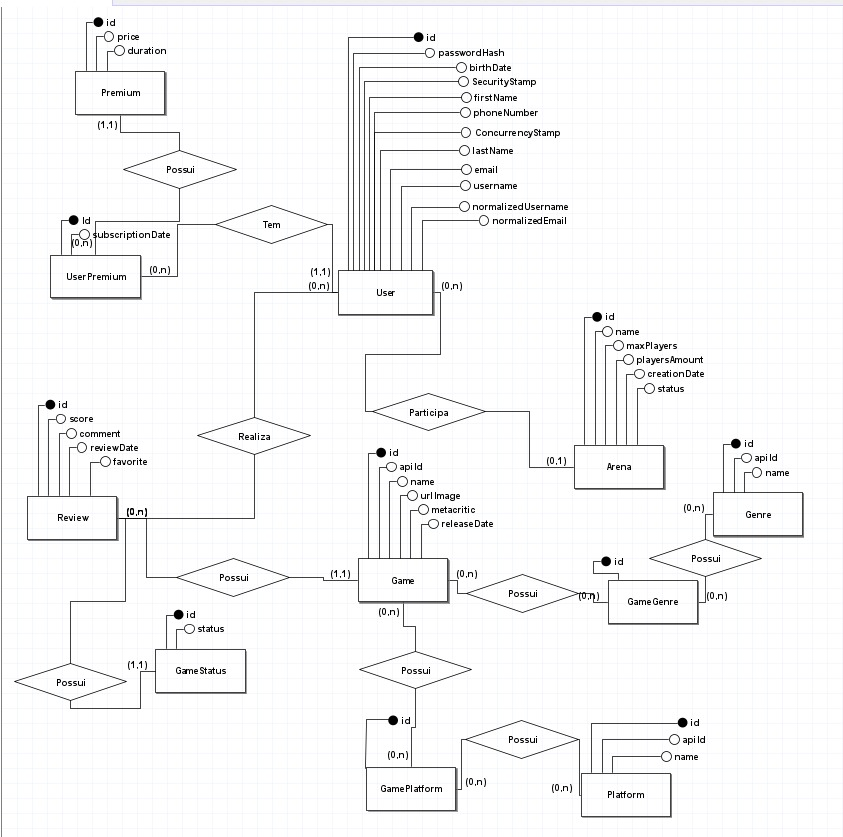
\includegraphics[scale = 0.50]{imagens/arquitetura/diagrama-mer.jpeg}	
%     \fonte{Os Autores}
% \end{figure}

\begin{sidewaysfigure}
    \centering
    \caption{Diagrama MER}
    \label{DiagramaMer}
    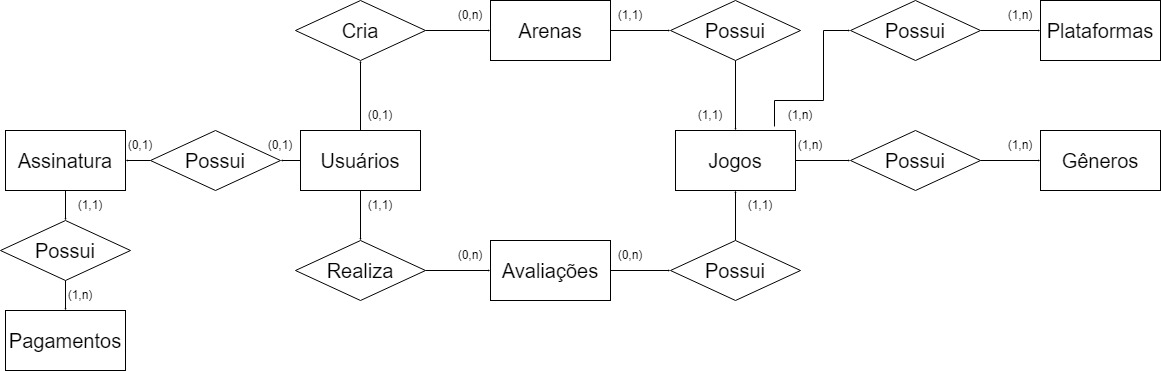
\includegraphics[scale=0.60]{imagens/arquitetura/diagrama-mer-new.jpg}
    \fonte{Os Autores}
\end{sidewaysfigure}

% Diagrama Entidade Relacionamento (DER)
\clearpage
\section{Diagrama Entidade Relacionamento (DER)}
A figura \ref{DiagramaDer} tem como objetivo representar com mais detalhes os atributos e relacionamentos das tabelas do banco de dados da aplicação.

\begin{sidewaysfigure}
    \centering
	\caption{Diagrama DER}
    \label{DiagramaDer}
    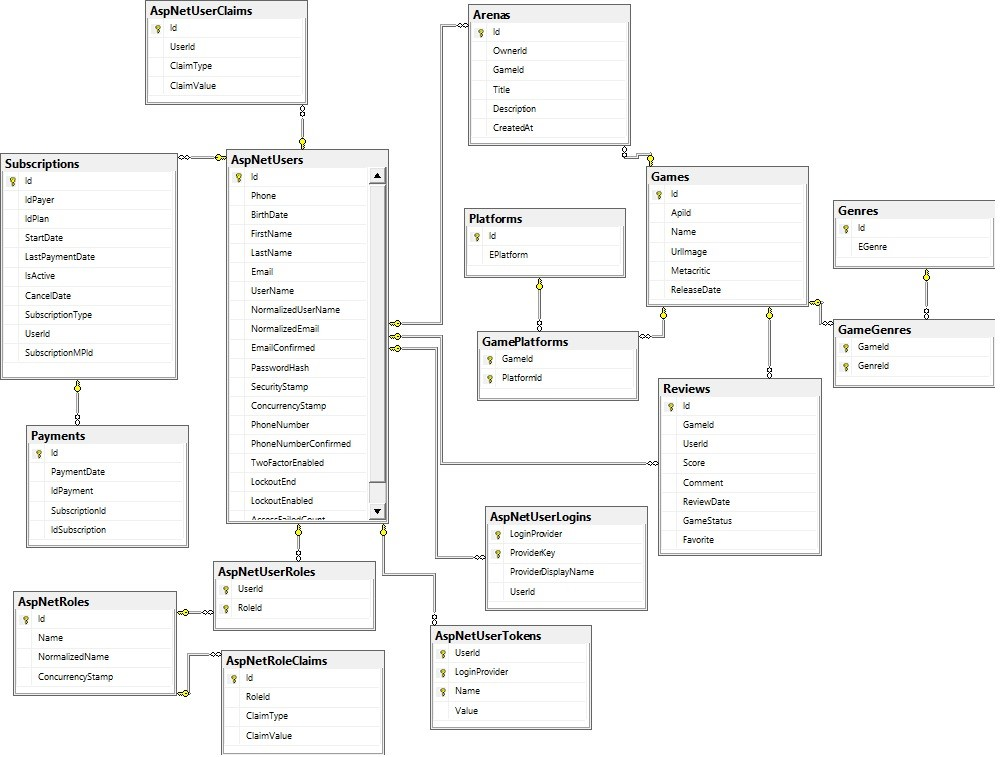
\includegraphics[scale =0.70]{imagens/arquitetura/diagrama-der.jpeg}	
    \fonte{Os Autores}
\end{sidewaysfigure}

% Volumetria
\clearpage
\section{Volumetria}

A volumetria configura-se como um conceito de relevância primordial no tocante à mensuração das dimensões e ao espaço apropriado que o repositório de dados de determinada aplicação ocupa. Além disso, reveste-se de caráter prospectivo ao possibilitar a estimativa da ocupação futura. Estas informações revestem-se de absoluta importância para a delineação adequada do projeto em si e do arcabouço informacional subjacente, o que ganha contornos ainda mais destacados em corporações de grande envergadura. Tal como pode ser constatado no Quadro \ref{volumetria}, o atual tamanho do banco de dados da aplicação \textit{GameLocker} é estimado em aproximadamente 16MB.

\begin{quadro}[thb]
\centering
\ABNTEXfontereduzida
\caption{Tamanho do Banco de Dados}

\begin{tabular}{|l|c|c|c|}
\hline
\thead{Name} & \thead{DB Size} \\
\hline
GameLockerdb & 16.00 MB \
\\\hline
GameLockerdb2 & 16.00 MB \
\\\hline
GameLockerdb3 & 16.00 MB \
\\\hline
\end{tabular}
\label{volumetria}
\fonte{Autores}
\end{quadro}
